% ==========================
% # Comunicação            #
% ==========================

\subsubsection{Comunicação/Divulgação}

A divulgação é, no nosso entender, um dos desafios mais importantes e difíceis de qualquer instituição. É através dela que podemos chegar ao público alvo que queremos. Dessa forma, achamos essencial uniformizar toda a imagem que é passada para fora bem como orientar todos os meios que dispomos de forma a destacar a informação que, de facto, mais necessita ser destacada. No nosso entender, a comunicação/divulgação é muito mais do que o trabalho de imagem, é sim a organização de toda a informação, material e calendarização do material a divulgar.

\paragraph{Separação do Pelouro da Comunicação e Imagem}
Pelos motivos referidos, no presente mandato, decidimos separar a Comunicação da Imagem. Por termos criado também um Pelouro novo, o Pelouro das Relações Externas, entendemos passar a componente de comunicação para este novo Pelouro, dado que, pensávamos nós, o trabalho do mesmo seria reduzido comparando com um Pelouro normal, principalmente no primeiro semestre, a altura mais difícil em qualquer alteração: a de habituação ao novo paradigma. É também de realçar que, anteriormente, o trabalho de divulgação de cada atividade era feito pelo Pelouro responsável pela organização do mesmo. Desta forma, um Pelouro mais ativo poderia divulgar uma atividade de uma forma excelente ou até exagerada enquanto que um Pelouro menos ativo nesta área poderia organizar uma atividade excelente sem se esforçar na divulgação da mesma e, assim, ter “a casa às moscas”. Algo que reparámos é que havia, portanto, uma discrepância enorme na divulgação dos diferentes eventos de cada Pelouro.

\paragraph{Comunicação/Divulgação no início do mandato}
No início do mandato, em junho, a divulgação começou a ser feita ainda pelo Presidente e Vice-Presidente do Núcleo, embora, note-se, a atividade fosse muito reduzida e a divulgação se tenha baseado na divulgação das atividades do mês e na divulgação da campanha de recolha de bens para os incêndios. Após todo o verão sem uma intervenção ativa do recém-criado Pelouro da Comunicação, iniciou-se a campanha de divulgação do apadrinhamento de Erasmus, algo que foi feito diretamente pelo Pelouro da Pedagogia, demonstrando de novo o problema referido acima. Assim, iniciaram-se conversações para que o Pelouro da Comunicação ficasse com o exclusivo da organização da divulgação do Núcleo. Durante todo o mês de setembro este Pelouro teve como responsabilidade criar um plano de divulgação, algo que já só fez em outubro. A tentativa de divisão de trabalho entre os vários membros da equipa foi outra das barreiras uma vez que a comunicação apresenta vários detalhes que são adquiridos com a experiência e, uma vez que o plano traçado implicava a mudança de responsável pela comunicação a cada semana (sendo que cada membro da equipa desse Pelouro só voltava a ter a responsabilidade semanal da comunicação do Núcleo passado mais de um mês) e uma vez que, caso algum membro falhasse, não havia nenhum plano B fez com que a atribuição da comunicação por completo a este Pelouro não resultasse. Em novembro, em reunião de CGs, foi discutido este tópico tendo-se definido novas regras, nomeadamente na emissão das imagens: a imagem passaria a fazer, sempre que se tratasse de um evento, um banner para evento de Facebook, um cartaz e um imagem retângulo para a televisão, quer os CGs pedissem isto ou não (esta premissa entrou de imediato em vigor tendo resultado sempre bem) e os CGs passariam a pedir a imagem um mês antes do evento sendo que a imagem devia divulgar a imagem feita com bastante antecedência para que houvesse algum feedback à mesma, correção de erros e tempo necessário para agendar a divulgação necessária (esta premissa nunca resultou uma vez que muitos dos CGs não pediam a imagem com antecedência nem o Pelouro da Imagem emitia sempre as imagens com muita antecedência em relação à data de divulgação). Por fim, no final de novembro, em nova reunião de CGs, decidiu-se que a comunicação passaria a ser gerida, em exclusivo, pelo Presidente e Vice-presidente do Núcleo, em conjunto, algo que aconteceu até ao final do mandato. De notar que, dada a carga de trabalho dos mesmos, isto não permitiu levar a comunicação a novas áreas nem permitiu uma pressão intensiva e necessária sobre os CGs para que estes fizessem os pedidos de imagem necessários a tempo. Já em maio, no final do mandato, após se saber que a Joana Dourado seria a próxima CG da Comunicação, integrou-se a mesma na equipa da comunicação passando também ela a tomar conta deste assunto.

\paragraph{Modelo de divulgação adotado}
Passamos agora a descrever o modelo de comunicação em que trabalhámos na maior parte do mandato, já após a estabilização da mesma.

\paragraph{Instagram}
No final de agosto de 2017, foi criado o Instagram do Núcleo. Todos os membros do Núcleo tinham acesso à password do Instagram. Desta forma, todos podiam colocar insta stories ou até publicações no mesmo quando se realizavam eventos, algo que, na nossa opinião, resultou muitíssimo bem. Por sua vez, a ideia do Instagram foi criar um perfil “amigo” dos nossos colegas. Assim, tentámos sempre não colocar cartazes nem imagens pré-feitas, mas sim fotografias e vídeos do que ia decorrendo fazendo assim um perfil “friendly”. Por sua vez, foi também incentivada a inserção de fotos e histórias em atividades fora \acrshort{neeec} como por exemplo, assembleias de núcleos e assembleias magnas. A divulgação do trabalho interno do Núcleo foi algo que também foi possível de fazer através do Instagram divulgando-se assim momentos de teambuilding, reuniões de pelouros, reuniões com outras entidades, entre outros.

\paragraph{Plano de divulgação}
A partir de novembro foi criado um plano de divulgação que incluía os seguintes campos: hora das divulgações, tipo e local da divulgação (por exemplo, publicação no grupo do Facebook do curso ou no Facebook do Núcleo, criação de evento ou publicação de cartaz, etc). Este plano integrava o Facebook e o Instagram, principalmente assentando no seguinte paradigma: qualquer pessoa com acesso aos meios de divulgação poderia fazer publicações desde que estas não coincidissem com o plano de divulgação (ou seja, por exemplo, não se poderia publicar no Instagram às 21h30 de um dado dia que se estava numa assembleia magna após se ter divulgado os vencedores de um torneio às 21h mas poderia-se publicar quando já tivessem passado, pelo menos, umas 5 horas da última publicação). O mesmo principio foi aplicado ao Facebook. Este plano começou por ser feito num Excel mas posteriormente migrou para o trello onde resultou muito melhor por ser de fácil utilização. Este canal do trello ficou aberto a todos os membros do Núcleo sendo identificados em cada cartão os responsáveis pela imagem, pela divulgação e pelo evento. Por sua vez, este canal do trello tinha integração com o Google calendário pelo que, quem quisesse, podia subscrever o calendário e ter assim na sua agenda todo o plano de divulgação.

Algo que nos foi explicado na formação do \acrshort{aac} (in)Forma e que viemos, ao longo do tempo, a notar que foi verdade, foi a importância de não deixar o Instagram mais do que um ou dois dias sem publicação e tentar não fazer mais do que uma publicação por dia no Facebook.

\paragraph{Excesso de divulgação}
Ao longo do ano deparámo-nos também com alguns problemas na divulgação provocados pelo facto de se ter tanta informação a transmitir quer pelo aumento de atividades do Núcleo, quer pelos vários pedidos de divulgação que nos chegam diariamente. Assim, tentámos restringir as publicações de ofertas de emprego, limitando-as ao email e ao grupo interno de Facebook.

\paragraph{Facebook: gostos e partilha de publicações}
No Facebook, sempre que era feita alguma publicação, era também importante fazer algum spam através de partilhas e likes nas publicações. Um problema grave com que nos deparámos é que os membros do Núcleo faziam poucos likes nas publicações fazendo com que as publicações não tivessem muitas interações. É também importante que as publicações que se esperam mais virais não sofram o mesmo tipo de spam que as publicações menos “interessantes” (por exemplo, a publicação sobre a remodelação dos espaços de estudo, sem qualquer tipo de partilha, rapidamente se tornou a publicação com mais likes e comentários de sempre na página de Facebook do \acrshort{neeec}). Em relação às partilhas, um problema que tivemos foi o facto de nem toda a gente partilhar em simultâneo as publicações. Algo que aprendemos também na formação do \acrshort{aac} (in)Forma e se revelou ser verdade foi a importância de todos partilharem ao mesmo tempo e o desinteressem em segmentar as partilhas numa escala horária pois o alcance da publicação não melhora com isso.

\paragraph{LinkedIn}
Por sua vez, criámos também um LinkedIn do \acrshort{neeec} onde pudemos contactar com algumas empresas. No entanto, o trabalho a fazer nesta plataforma é ainda muito grande, algo que recomendamos que seja feito no futuro, principalmente para eventos com elevada relação com as empresas.

\paragraph{Outras redes sociais}
O \acrshort{neeec} também tem presença em várias outras plataformas sociais:
\begin{itemize}
\item Twitter\\
A presença nesta rede é já antiga sendo publicado tudo aquilo que é publicado no Facebook, de forma automática. Além deste mecanismo, não fizemos mais nenhuma interação nesta rede social.
\item Snapchat\\
No mandato anterior foi criado um Snapchat do Núcleo, algo que teria o mesmo objetivo do Instagram. Contudo, ao longo desse mandato o Snapchat foi utilizado muito poucas vezes uma vez que quem utilizava a app tinha de fazer logout da sua conta para fazer login na conta do Núcleo, ao contrário do que sucede com o Instagram. Desta forma, a plataforma foi abandonada este mandato mas recomendamos uma avaliação sobre a possibilidade de dinamizar a conta do Núcleo nesta plataforma de novo.
\item YouTube\\
A presença do Núcleo nesta conta tem sido diminuta até porque os vídeos são cada vez mais divulgados diretamente no Facebook ou no Instagram. Contudo, é de notar que no youtube os vídeos ficam públicos para qualquer pessoa com acesso à internet e não apenas para quem tem acesso às plataformas referidas pelo que recomendamos uma dinamização da mesma no futuro.
\end{itemize}

\paragraph{Colocação de cartazes}
Quanto aos cartazes, o \acrshort{neeec} dispõe de vários locais para afixar cartazes (entrada do piso 2, junto ao elevador da torre B no piso 2, na zona do bar, na sala de estudo do piso 6 e na sala de convívio). Estes espaços foram quase todos arranjados pelo \acrshort{neeec} este ano ficando em falta um local de divulgação na zona do piso 4 da torre T, prometido pelo Departamento para breve. Na zona da sala de estudo, era também interessante ter um ponto de divulgação logo à entrada, local por onde passam diariamente inúmeros estudantes. Por sua vez, a zona da entrada do piso 2 é de escassa visualização, principalmente pelo exagero de cartazes lá presente sobrepostos por expositores. A zona da máquina de café do piso 2 seria também um ponto de divulgação interessante a implementar no futuro. A afixação dos cartazes e organização destes espaços era feita pelo Secretário do \acrshort{neeec}, uma vez que o trabalho de comunicação estava em cima da Direção, contudo achamos que no futuro deve ser feito pelo Pelouro da Comunicação pois a distribuição de um trabalho que diz respeito ao mesmo assunto por tanta gente diferente só trás mais entropia desnecessária.

\paragraph{Divulgação via email}
Além destes meios existe ainda a divulgação via email que pode ser feita por três vias:
\begin{enumerate}
\item Inforestudante\\
Através de um pedido de envio à Secretaria do \acrshort{deec}, nomeadamente à Maria João Cavaleiro, é possível enviar notificações via inforestudante para todos os alunos da \acrshort{uc}, através dos filtros que bem entendamos. Contudo, este meio, por ser o mais privilegiado, não deve ser transformado em spam como tem vindo a acontecer por outras instituições, nos últimos tempos. Assim, decidimos só enviar informações essenciais como convocatórias de plenários (obrigatório o envio por esta forma, segundo o nosso Regulamento Interno) e informações sobre eleições dos delegados de ano e informações sobre o mapa de avaliações. Adicionalmente enviámos também informação sobre a reestruturação de curso, a semana dos ramos e o Bot Olympics.

\item Email direto via ucxxxxxxxxxx@student.uc.pt\\
É possível enviar diretamente email para os estudantes através do endereço indicado. Enviando emails desta forma, os emails vão para o email de cada aluno, associado ao InforEstudante pelo que, a probabilidade de os receberem é quase de 100\%. Este meio foi utilizado para divulgar, por exemplo, os códigos da parceria com a drag \& print que tiveram de ser diferentes para cada aluno.

\item Listas all users\\
Este é sem dúvida o meio, via email, que menos chega aos estudantes. Desta forma, foi só usado para enviar informação pouco interessante mas obrigatória.
\end{enumerate}

\paragraph{Passa-palavra}
Por fim, mas não menos importante, falamos do passa-palavra. Este é, e continua a ser, o meio de divulgação mais importante do Núcleo. É essencial fazer com que todos os membros do Núcleo se sintam à vontade e entusiasmados em incentivar os seus amigos mais próximos a vir às atividades do Núcleo. Esta é, sem dúvida, a tarefa mais árdua da comunicação.

\paragraph{NEEEC Informa}
Existem ainda informações a publicar que costumam sair sem imagem (horários, por exemplo) pelo que o Pelouro da imagem criou um template chamado “\acrshort{neeec} Informa” que está disponível para utilizar facilmente (sendo, no entanto, necessário o programa Illustrator para editar o texto, a cor e/ou a imagem). Este template tem vindo a ser utilizado para informações nos últimos tempos e as publicações têm obtido um alcance mais elevado do que era costume.

\paragraph{Hall of Fame}
Foi também nosso objetivo criar uma "Hall of Fame"\space para que fosse possível divulgar alguns dos feitos de músicos, atletas, entre outros do nosso Departamento. Esta ideia acabou por nunca avançar uma vez que já nos aproximávamos do final do mandato quando a mesma se encontrava pronta. Adicionalmente é possível divulgar muita informação sobre investigação no Departamento, novidades na área da engenharia eletrotécnica pelo que sugerimos uma forte colaboração entre o Departamento e o Núcleo para a criação de novos meios de divulgação massiva como a televisão e um possível jornal.

% ==========================
% # TV do \acrshort{deec}             #
% ==========================

\paragraph{TV do \acrshort{deec}}

O \acrshort{deec} tem televisões distribuídas pelo Departamento (nomeadamente no bar e na entrada do piso 2) onde é possível passar alguma informação nomeadamente notícias (em texto) e anúncios (em imagem). O \acrshort{neeec} costumava pedir à D. Ana Maria Bernardes para colocar informação (em texto) nestas televisões de forma a publicitar os seus eventos. Este processo repetia-se para as atividades de maior dimensão apenas. Após conversações com o GRI, o \acrshort{neeec} passou a ter uma conta de acesso à plataforma que permite a inserção dos dados nas televisões (http://cptv.streamline.pt/\#/login) passando, desta forma, o \acrshort{neeec} a fazer também a gestão da televisão. Adicionalmente, o \acrshort{neeec} incentivou o \acrshort{gri} a criar uma nova funcionalidade na plataforma que permite a inserção de imagens (1040 x 840 pixeis) passando assim a ser possível inserir imagens como se pode ver na figura \ref{fig:tvDEEC1}.

\begin{figure}[ht]
\centering
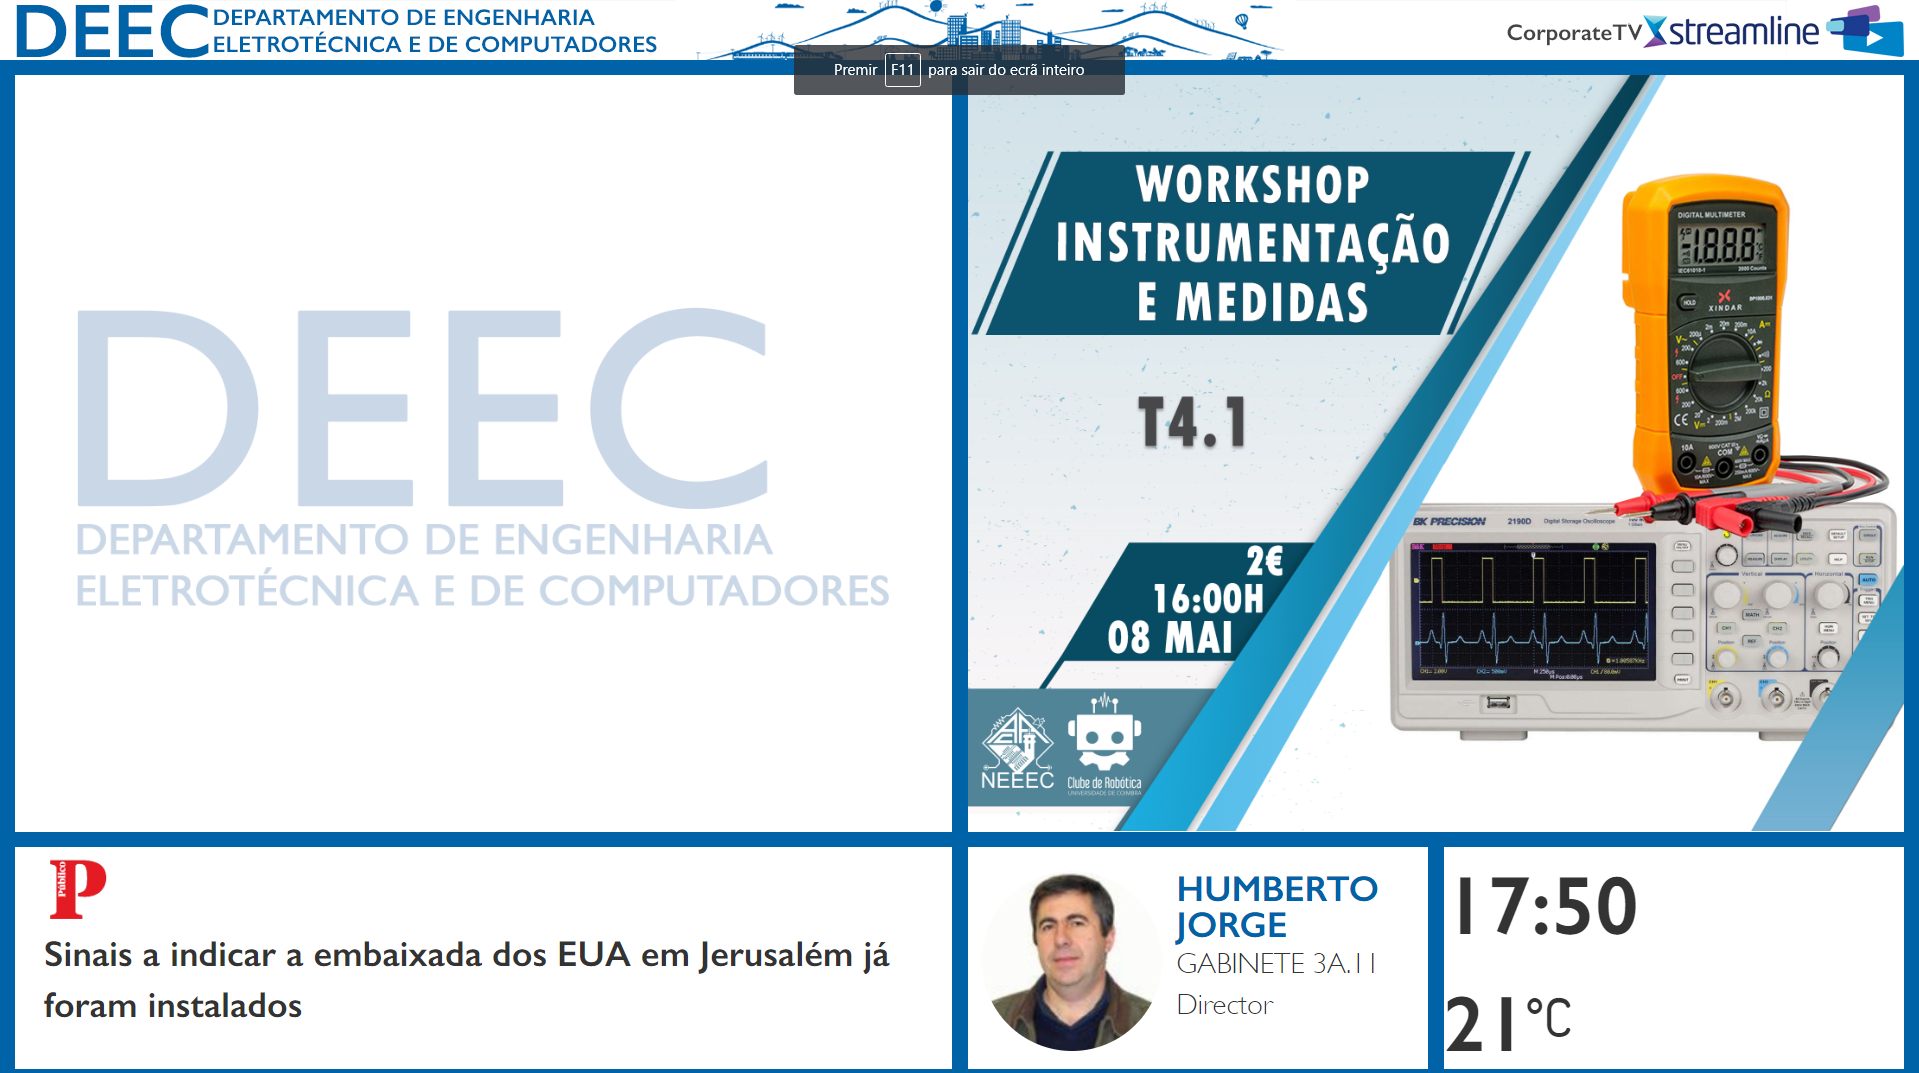
\includegraphics[width=\textwidth]{imagens/tvDEEC1.png}
\caption{Layout antigo.}
\label{fig:tvDEEC1}
\end{figure}

Adicionalmente, após umas obras de remodelação da sala de reuniões do \acrshort{deec}, o professor Humberto Jorge ofereceu uma televisão ao \acrshort{neeec}. Esta televisão foi instalada na sala de convívio tendo também sido instalado um pc que permite a exibição do layout das tv’s do \acrshort{deec} nesse ecrã. O GRI, gentilmente, criou um novo layout específico para o \acrshort{neeec} que ficou em exibição nessa televisão e pode ser visto na figure \ref{fig:tvDEEC2}.

\begin{figure}[ht]
\centering
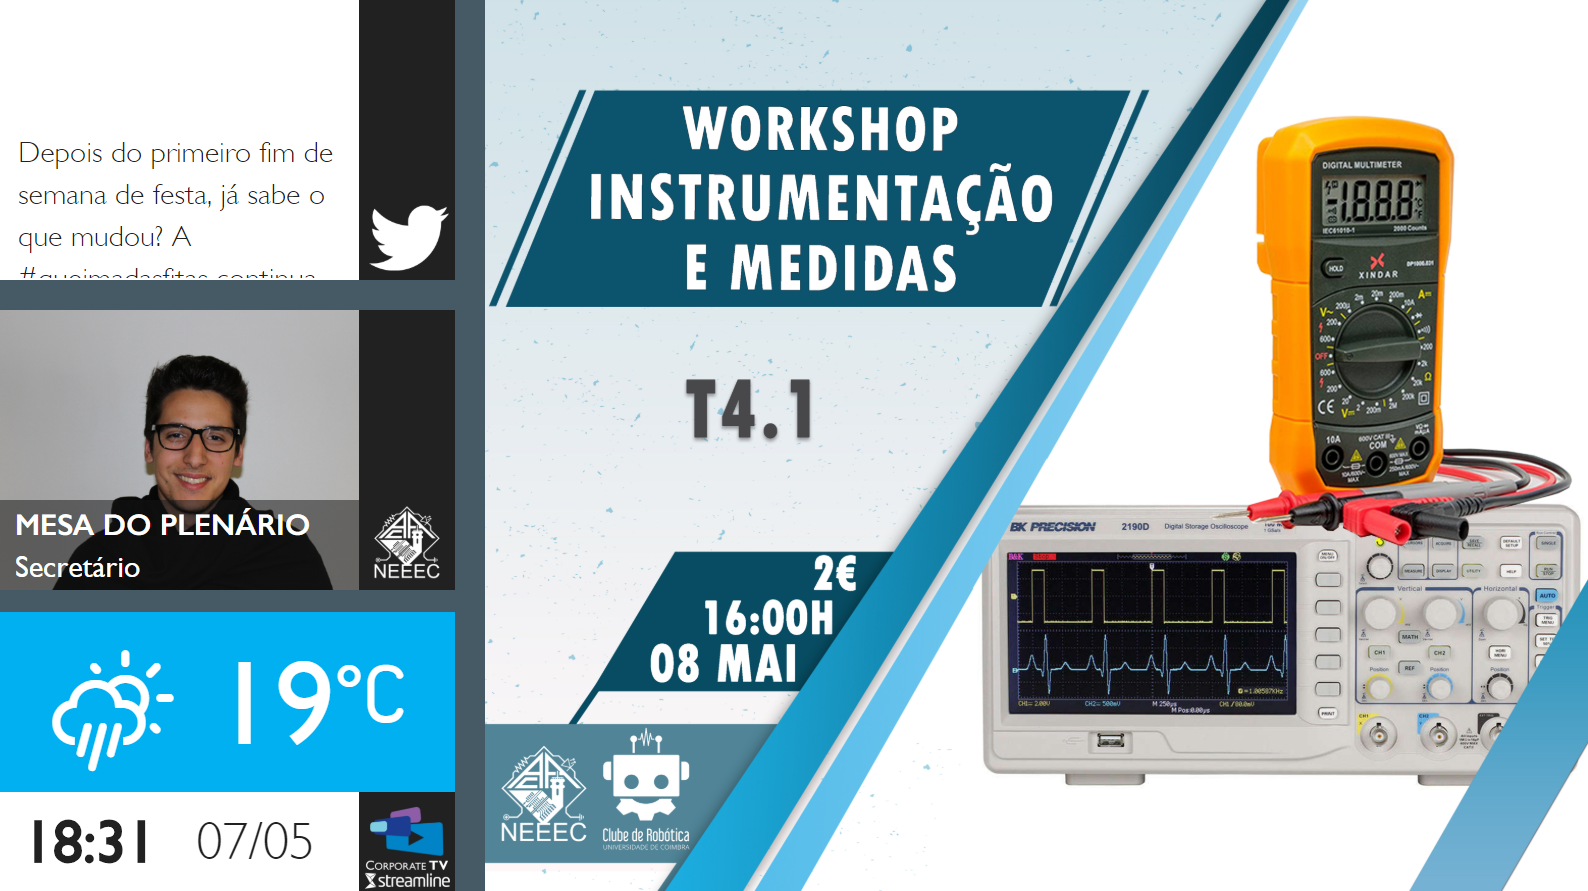
\includegraphics[width=\textwidth]{imagens/tvDEEC2.png}
\caption{Layout criado para o \acrshort{neeec}.}
\label{fig:tvDEEC2}
\end{figure}

Todos os layouts são totalmente configuráveis na plataforma onde se inserem as imagens. As fotos, nomes e cargos dos membros do \acrshort{neeec} que aparecem na tv, podem ser alterados através de um ficheiro que se encontra no servidor onde está alojado o site do \acrshort{neeec}.

\begin{itemize}
\item Inserir imagens/notícias na plataforma:
	\begin{itemize}
	\item Aceder a http://cptv.streamline.pt/\#/login;
    \item Selecionar o ícone de editar ao lado de \acrshort{fctuc} | Departamento de Eng. Eletrónica e de Computadores;
    \item Descer até à secção de imagens e clicar em “Upload de imagens”;
    \item Escolher o(s) ficheiro(s) a enviar;
    \item Ir à galeria de imagens, selecionar a foto que se pretende colocar na notícia e pressionar em “Copiar URL”;
    \item Selecionar “Voltar à edição” e ir à área de notícias, selecionando o ícone do balão de fala para adicionar uma nova notícia;
    \item Caso se pretenda inserir apenas uma imagem, selecionar, no tipo, “Imagem” e colar o URL da imagem no campo devido. Colocar um título na notícia (não irá ser mostrado);
    \item Escolher a data (após a data selecionada como data de fim a notícia irá deixar de estar visível nas televisões);
    \item Carregar em alterar;
    \item Para inserir uma notícia de texto basta, no tipo, selecionar “Informação”. Neste modo é também possível inserir imagens devendo-se proceder da mesma forma para copiar o URL da imagem. Deve-se depois, no campo “Conteúdo”, selecionar o ícone de imagem e colocar a foto que se pretende, dimensionando também o tamanho e escolhendo a posição da imagem no ecrã.
	\end{itemize}
\end{itemize}

Este meio veio facilitar o nosso trabalho por permite a inserção de textos, vídeos e imagens com uma data de início e uma data de fim de divulgação que poderá ser posterior à atual. Desta forma, a imagem ao criar a imagem dos eventos enviava sempre uma imagem para o formato da tv sendo assim possível inseri-la no sistema e ter mais um meio de divulgação que funciona bastante bem, de forma fácil, uma vez que é tem uma divulgação dinâmica e está sempre organizado de forma automática.

% ==========================
% # Notas de Imprensa      #
% ==========================

\paragraph{Notas de Imprensa}

Ao longo do ano existem várias atividades que poderão ser divulgadas facilmente através da imprensa, nomeadamente a regional. Desta forma, achamos que deveria existir alguém no Núcleo designado para ser assessor de imprensa, contudo, novamente pelos problemas referidos sobre o Pelouro das Relações Externas e Comunicação, tal nunca foi feito. Ao longo deste ano, esta tarefa foi feito essencialmente pela Presidência e pelo André Duarte, no caso do Bot Olympics.

Para uma melhor divulgação das notícias é possível entrar em contacto com a assessoria de imprensa da \acrshort{uc}, atualmente gerida pela Dr.ª Cristina Pinto, que facilmente ajuda o \acrshort{neeec} na divulgação de todas as notícias. Foi também possível entrar em contacto com a \acrfull{ruc} e o Jornal "A Cabra", através dos formulários disponíveis nos seus sites, bem como com o "Notícias de Coimbra"\space através do email fernandomoura@noticiasdecoimbra.pt. Ao longo do ano foram sendo sempre criadas \textit{press releases} (como aconteceu na \acrshort{f3e}, no \acrshort{ene3} e no aniversário do Núcleo, por exemplo) que eram divulgados junto das entidades. Mais tarde, os jornais interessados ou vinham ao \acrshort{deec} fazer entrevistas presenciais ou faziam-nas por via telefónica.

% ==========================
% # Ligação C&I e Pelouros #
% ==========================

\paragraph{Ligação C\&I e Pelouros}

A ligação entre a imagem, a comunicação e os diversos pelouros e comissões organizadoras do \acrshort{neeec} foi um dos nossos maiores desafios. Para tal foram criadas várias soluções para este problema:
\begin{itemize}
\item Foi criado um formulário de pedidos de imagem que os Coordenadores deveriam preencher quando querem pedir algo à imagem. Este formulário, uma vez que tinha várias perguntas diretas, fazia com que não fossem esquecidos pormenores importantes que é normal serem esquecidos como, por exemplo, quais as entidades que colaboram com o \acrshort{neeec} nessa atividade e devem aparecer no cartaz.
\item Sala feedback divulgação no Slack: esta era uma sala onde estavam presentes todos os membros da imagem, da comunicação e os CGs dos diversos pelouros sendo o local onde a imagem enviava as versões finais provisórias dos seus trabalhos. Desta forma, todos poderiam corrigir algum erro e opinar sobre a qualidade das imagens, algo que foi muito positivo para a emissão do material a divulgar em concordância entre todos os envolvidos.
\end{itemize}